\newpage
\section{Introduction}
\label{sec:introduction}
\vspace{4.5mm}
% state the learning objective
\par In this laboratory assignment, a circuit containing two voltage sources (independent source $V_a$ and current controlled source $V_c$), and two current sources (independent source $I_d$ and voltage controlled source $I_b$), connected to multiple resistors (from $R_{1}$ to $R_{7}$), is going to be studied. The described circuit can be observed in detail in Figure~\ref{fig:rc}.
\vspace{3mm}
\par Although the circuit is composed by somewhat simple, linear components, these are the core of electronic circuits. Because of that, it is essential for one to understand the way they behave to be able to build and apply their knowledge in other more complex circuits. Therefore, its study is still of maximum importance. 
\vspace{3mm}
\par In Section~\ref{sec:analysis}, a theoretical analysis of the circuit - using the mesh and nodal methods - is presented. After that, in Section~\ref{sec:simulation}, the circuit is analysed via simulation, using the software Ngspice. The obtained results are then compared, explaining the reasons behind the differences and similarities found. Finally, one can find the conclusions of this study outlined in Section~\ref{sec:conclusion}.

\begin{figure}[h] \centering
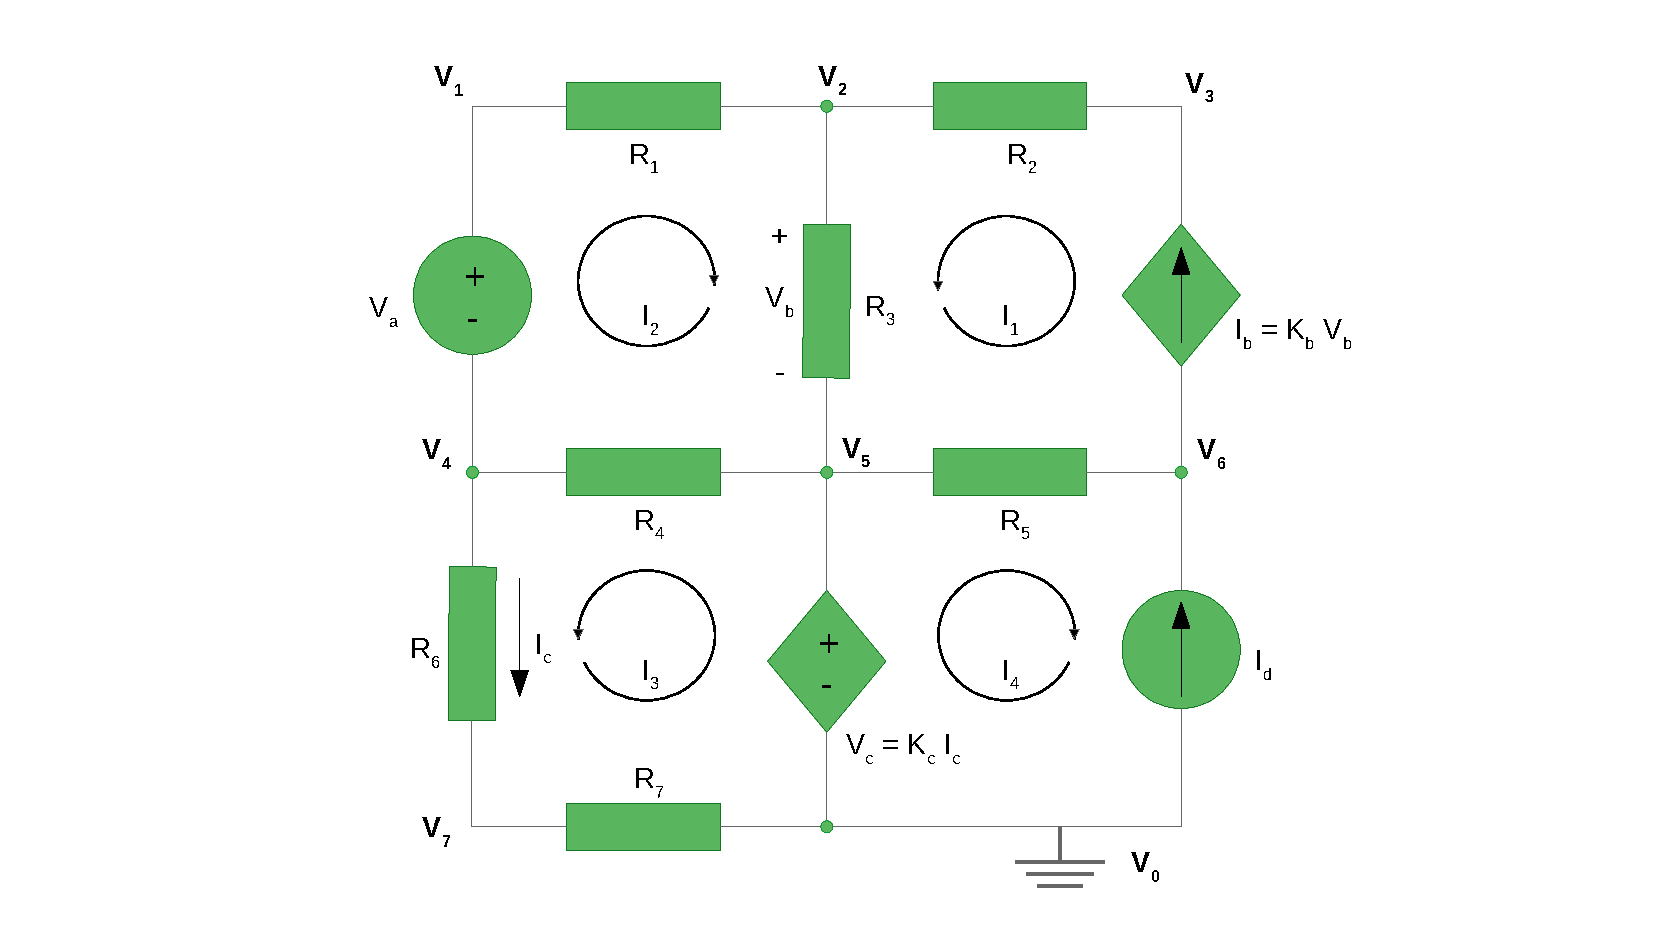
\includegraphics[scale=0.5]{rc.pdf}
\caption{Circuit diagram with node ($V_0$ to $V_7$) and mesh current ($I_1$ to $I_4$) representation.}
\label{fig:rc}
\end{figure}
